%% -*-LaTeX-*-
%%
%% This manuscript has been written using the IEEEtran macros
%%
%% (c) 2021 Grupo AIA, RTE  
%%
%% 
%%

\documentclass[conference]{IEEEtran}
\usepackage[utf8]{inputenc}
\usepackage{hyperref}
\usepackage{graphicx}
%\usepackage{amsmath,amssymb,amsfonts}
%\usepackage{booktabs}
\usepackage{cite}
\usepackage[cbgreek]{textgreek} % Only for Dynawo "omega" font
\usepackage{listings}
\usepackage{fancyvrb}
\usepackage{xcolor}



%%%%%%%%%%%%%%%%%%%%%%%%%%%%%%%%%%%%%%%%%%%%%%%%%%%%%%%%%%%%%%%%%%%%%%%%%%%%%%%
%% Our short-hand macros
\newcommand{\Dynawo}{Dyna\textomega o} % unfortunately, it doesn't show in bold
\newcommand{\TODO}{\texttt{TODO:}}

%% Our colors for backgrounds and code listings
\definecolor{light-gray}{gray}{0.9}
\definecolor{dark-gray}{gray}{0.4}
\definecolor{light-blue}{RGB}{64,64,255}
\definecolor{dark-blue}{RGB}{16,16,64}

%% Our config parameters for code listings
\lstset{
  language=Python,
  backgroundcolor=\color{light-gray},
  basicstyle=\scriptsize\ttfamily,
  keywordstyle=\bfseries,
  identifierstyle=,
  stringstyle=\itshape,
  showstringspaces=false,
  commentstyle=\color{dark-gray}
}

%% Our short-hand macros for code snippets: \console and \code
\lstnewenvironment{console}{\lstset{language=bash}}{}
\newcommand{\code}[1]{\texttt{#1}}

%% More sane colors for hyperref links
\hypersetup{
  colorlinks = true, % color links instead of ugly boxes
  urlcolor   = blue, % color of external hyperlinks
  linkcolor  = dark-blue, % color of internal links
  citecolor  = red   % color of citations
}





%%%%%%%%%%%%%%%%%%%%%%%%%%%%%%%%%%%%%%%%%%%%%%%%%%%%%%%%%%%%%%%%%%%%%%%%%%%%%%%%
\begin{document}

\title{Development of an Open Source Tool to Compare Simulators on Large-Scale Cases - Application on Dyna$\omega$o}% A proposal for a new title
%\title{Black-box validation and A/B testing of large-scale cases with DynaFlow and DynaWaltz simulators}


\author{
  \IEEEauthorblockN{
    José Luis Marín\IEEEauthorrefmark{1},
    Vicenç Gaitan\IEEEauthorrefmark{1},
    Guiu Oms\IEEEauthorrefmark{1},
    Adrien Guironnet\IEEEauthorrefmark{2},
    Quentin Cossart\IEEEauthorrefmark{2},
    and Marco Chiaramello\IEEEauthorrefmark{2}}
  \IEEEauthorblockA{
    \IEEEauthorrefmark{1}Aplicaciones en Informática Avanzada SL\\
    Avda. de la Torre Blanca, 57 (Ed.\ EsadeCreapolis)\\
    08172 -- Sant Cugat del Vallès, Spain\\
    Email: \{marinjl, gaitanv, omsg\}@aia.es
  }
  \IEEEauthorblockA{
    \IEEEauthorrefmark{2}RTE R\&D department\\
    7C place du Dôme, 92073 Paris La Défense Cedex\\
    Email: \{adrien.guironnet, marco.chiaramello, quentin.cossart\}@rte-france.com
  }
}

\maketitle

% Remember: no symbols, special chars, footnotes, or math in Title or Abstract
\begin{abstract}
  Dyna$\omega$o is an open source hybrid Modelica/C++ suite of simulation tools for power systems, geared
  towards the dynamic simulation of large transmission networks at different
  time scales, from the steady-state calculation to transient stability analysis. In this paper we present a set of open source tools designed for: (a)
  validation of Dyna$\omega$o based on black-box testing against existing established
  simulators, or against previous validated versions of Dyna$\omega$o; (b) exploration
  and analysis of the effects of modelling changes and model parameters on the
  network response, by means of A/B testing. In both cases the methodology is
  based on the automatic generation of an extensive set of cases derived from a
  given base case, typically by means of N-1 contingencies. These tools, based
  on Python and Jupyter Notebooks, are designed with flexibility in mind, in
  order to provide easy ways to change and adapt the code to future testing
  scenarios.
\end{abstract}

\begin{IEEEkeywords}
  steady state calculation, dynamic simulation, blackbox validation
\end{IEEEkeywords}




%%%%%%%%%%%%%%%%%%%%%%%%%%%%%%%%%%%%%%%%%%%%%%%%%%%%%%%%%%%%%%%%%%%%%%%%%%%%%%%%
\section{Introduction}

\Dynawo{}\cite{Guironnet18} is a suite of tools for the dynamic simulation, at
different time resolution levels, of modern power networks. It has been mainly
developed by RTE, and then released as open source under the umbrella of the
Linux Foundation Energy \textcolor{red}{Not in the LFE yet, so we can remove the mention}.  Its design is based on two major guiding principles:
the use of a high-level modelling language (Modelica \textcolor{red}{maybe put a reference presenting the language}) and a strict separation
between the modelling and the solving mechanisms.  Its implementation brings to
the table a novel hybrid approach that combines the power of declarative,
computationally acausal modelling (also referred to as equation-based modelling)
with certain high-performance C/C++ modifications that take advantage of the
specific optimization opportunities available in large power networks (such as,
for instance, the extensive work on high-performance DAE solvers for these
highly sparse systems).  \Dynawo{} thus aims at providing power system
stakeholders with a next-generation of open source simulation tools that overcome the
limitations of legacy closed-source programs, while being performant enough to
be used in production settings at large transmission operators. The key goals
are transparency and flexibility of modelling, which will result in robustness
and interoperability. It is hoped that this will enable an effective
collaboration and cooperation in the power system community, something that has
been difficult to achieve with legacy commercial tools.  For a recent update on
\Dynawo{} developments, see the presentation \cite{Guironnet21} or consult the
official website~\cite{Dynawo}.



\subsection{Objectives of the developed comparison tools}
%\subsection{Aims: not just validation}

%% Stress the possibilites offered by the tool to validate or observe the
%% influence of one parameter or model change on the system reponse, in a
%% systematic way.

Validation of dynamic simulators is hard, and it obviously starts at the level
of individual device models. But, since these devices are increasingly more
complex (with lots of new power electronics and sometimes governed by
algorithmic controls), one needs whole-system functional testing in order to
assess the behavior on complete network cases. As in any hierarchical
system-of-systems, it is not always evident how the lower-level details (device
model choices, parameters, etc.)  affect the behavior of the whole network. This
sort of testing is necessarily ``black-box'' in style, since there is no
systematic way to link the knowledge of the lower-level modelling to the behavior
of the higher-level, other than running simulations---in a certain limited
sense, what we have here is an ``emergent behavior''.  Therefore this sort of
black box simulations are not only useful for validating the software against
previous legacy simulators, or against new versions of the software, but also
for exploring and assessing the effects of different model choices, model
parameters, solver parameters, etc., on the behavior of the whole network,
\emph{in a systematic way}.

The tools presented here aim to fulfill this double role. They leverage modern
rapid development tools from the Python ecosystem (Pandas and Jupyter notebooks,
among many others) to accomplish this. They can automatically create and
configure extensive sets of test cases derived from a given base case, and
efficiently manage large amounts of output. Initially developed for the
validation of \Dynawo{} at the functional level, they are now also used for the
generation and exploration of extensive sets of cases. These are designed for a
couple of settings: long-term stability studies, with DynaWaltz, and steady state calculation studies, with DynaFlow. We also
report on our early experience using these on recent versions of \Dynawo{} and
several large network cases (actual cases from RTE's operational environment,
used for stability studies). Let us now briefly describe the aims and scope of
the tools in each of these two cases.



\subsection{DynaWaltz}

\Dynawo{} is flexible enough to accommodate several time scales: from sub-second
near-EMT (electro-magnetic trainsients)~\cite{Masoon21}, to long-term stability,
to steady-state calculation~\cite{Cossart21} studies. DynaWaltz is the \Dynawo{} tool used for long-term stability studies,
where the time scales are measured in minutes and the typical time steps can be
of the order of a few seconds. Used in this mode, \Dynawo{} simulates the grid
in the so-called quasi steady state, and contains most models impacting the
system slow dynamics: tap-changers, loads, static var compensators, etc.; as
well as secondary voltage regulation and special protection schemes. It is mostly used to study voltage collapses.

Long-term stability studies are a core process of transmission operation whose
role is ensuring power system stability: they consist in analyzing whether the
slow dynamics of the system could lead to an instability or a system
collapse. The validation tools described here were developed to assess and
validate DynaWaltz quantitatively and in a systematic manner, using RTE's
national grid models and cases. DynaWaltz is scheduled to be deployed in
production at RTE (in progressive stages that will start by end of 2021), for
$n$-day ahead operational security studies.

Initially, our overall approach was the use of another well-established
simulator, Astre, which is the currently used tool at RTE for long-term stability studies, as the reference for comparison and assessment. More
specifically, the validation efforts were focused on the results obtained for
the behavior of the coordinated Secondary Voltage Control systems. Shortly
after, the tools were extended to accommodate the comparison between different
Dyna$\omega$o versions, or between variations of case models, model parameters, and
solver parameters.



\subsection{DynaFlow}

DynaFlow~\cite{Cossart21} is a novel approach to the calculation of steady states
that leverages the \Dynawo's flexibility for modelling the dynamics at different
time scales. It overcomes an inherent problem that all static power flows have
when presented with controls: discrete event actions, dead-bands, and regulation
limits (control type-switching) all conspire to produce several possible
steady-state solutions, many of them operationally valid.  Static power flows
arrive at a single solution by means of several ``outer loops'' in which
heuristics (accumulated over years of practice) drive the choice of control
changes. However, these heuristics are not bullet-proof (for instance, one may
encounter ``hunting'' oscillations, even with standard tap changers); and more
importantly, they do not take into account the time constants and actual
dynamics of each control. Therefore, even the most pricipled approaches from the
static power flow camp, such as those based on optimization\cite{Ju20},
complementarity constraints~\cite{Murray15}, or HELM~\cite{Trias18} cannot
guarantee arriving at the correct solution, since they are blind to the the
different dynamics of different competing controls.

In the current scenario, where more complex power electronic devices and complex
algorithm-based controls are being introduced each year, this problem is getting
worse. DynaFlow solves these types of problems by simulating the network in the
time domain and using the actual time constants that govern the actions of
relevant controls. It also contemplates protection schemes, including modern
Special Protection Schemes (SPS), thus opening the door to the realistic
simulation of cascading effects in contingency studies and interactions between controllers.

Following the work done for DynaWaltz validation, we built a similar set of
tools for the validation of DynaFlow, as well as the exploration of extensive
sets of (contingency) cases.  Again, the approach to validation is based on
comparison against a well-established power flow, Hades 2, which is the currently used tool at RTE for steady state calculation. But in
addition, the tool is also prepared for comparing different DynaFlow versions,
and more generallly for assessing the effects of varying the case models, model
parameters, and solver parameters.


%%%%%%%%%%%%%%%%%%%%%%%%%%%%%%%%%%%%%%%%%%%%%%%%%%%%%%%%%%%%%%%%%%%%%%%%%%%%%%%%
\section{Structure and workflow}

\begin{center}
  \itshape
  Outline:
  \begin{itemize}
    \item High-level structure of the tools: preparatory steps, pipeline,
          analysis/exploration of outputs.
    \item Preparatory steps: the BASECASE. Requirements and other conventions
          assumed.
    \item Pipeline: general structure and steps involved. Design
          decisions. Parallelization. Storage Considerations.
    \item Analyzing the results: Jupyter notebook; output of metrics to
          file for further analysis with other tools.
    \item Other stuff: auditability of results (logs); reconstructing
          cases from the basecase and reproducing runs. Example: grepping for
          common modes of failure in log files --> uncover systematic problems
          appearing in a specific model, for instance.
    \item Typical workflows (for instance, start small with a small random
          sample of contingencies; then ramp up to full N-1 list. Or settle on
          a custom list of ``most interesting'' contingencies via regexes.)
    \item \textbf{Fig} of the block architecture for all this.
  \end{itemize}
\end{center}


Here follows a high-level description of the structure of the tools, along with
the typical workflow that the user is expected to carry out when using them.
For the details on installation instructions and its requirements, please refer
to the software documentation on the github repository, which is to be located
under the main Dyna$\omega$o project pages~\cite{DwoGitRepos}.

As described above, this validation system is based on comparing results against
a well-known reference system, the Astre simulator for the validation of DynaWaltz, and Hades 2 for the validation of DynaFlow. The cases used for
comparison are essentially all possible single-element disconnections (shunts,
lines, etc.). Therefore the tools are currently oriented towards the generation of
contingency cases derived from a given base case. However, the design is quite
modular; it is easy to modify the corresponding scripts so that the set of cases
would be something other than contingencies, such as, for instance, variations
of a given set of model parameters, or the solver timestep, etc.

%% to review further

The basic workflow of this system, from a functional point of view, is
as follows:
\begin{enumerate}
  \item Obtain a study case containing matching DynaWaltz/DynaFlow and Astre/Hades 2 files
        (in a standard file structure, see below)
  \item Prepare the base case: standardize the XML format and
        standardize the curves to be extracted;
  \item Create the contingency cases derived from the base case;
  \item Run Astre/Hades 2 and DynaWaltz/DynaFlow on the contingency cases, collecting logs;
        and results into organized (and compressed) storage
  \item Extract result data in a format common to Astre/Hades 2 and DynaWaltz/DynaFlow
        (this is for automata events, as curves have already been
        standardized in step 2);
  \item Compute metrics on the results obtained (both for curves and
        selected automata events);
  \item Use the Jupyter notebook to browse and analyze the results,
        and obtain lists of contingency cases that can be ranked according
        to various compound scores built on those metrics;
  \item Further analysis is possible using the ranked tables that the
        notebook exports to CSV files (e.g. using Excel).
\end{enumerate}

The study case (Step 1) is the main input to this whole process, and it is
required to satisfy a minimum set of requirements (discussed below), along with
other technical requirements.

Beginning with Step 2, this whole workflow has been automated with a series of
Python programs and Bash shell scripts. Tied together, we will refer to this
system as the \emph{process pipeline} for validation. This is depicted
schematically in Figure~\ref{fig:pipeline1} below.  In the following we describe
this pipeline in detail and explain how to run it either automatically or
manually step by step.

\begin{figure}
  \centering
  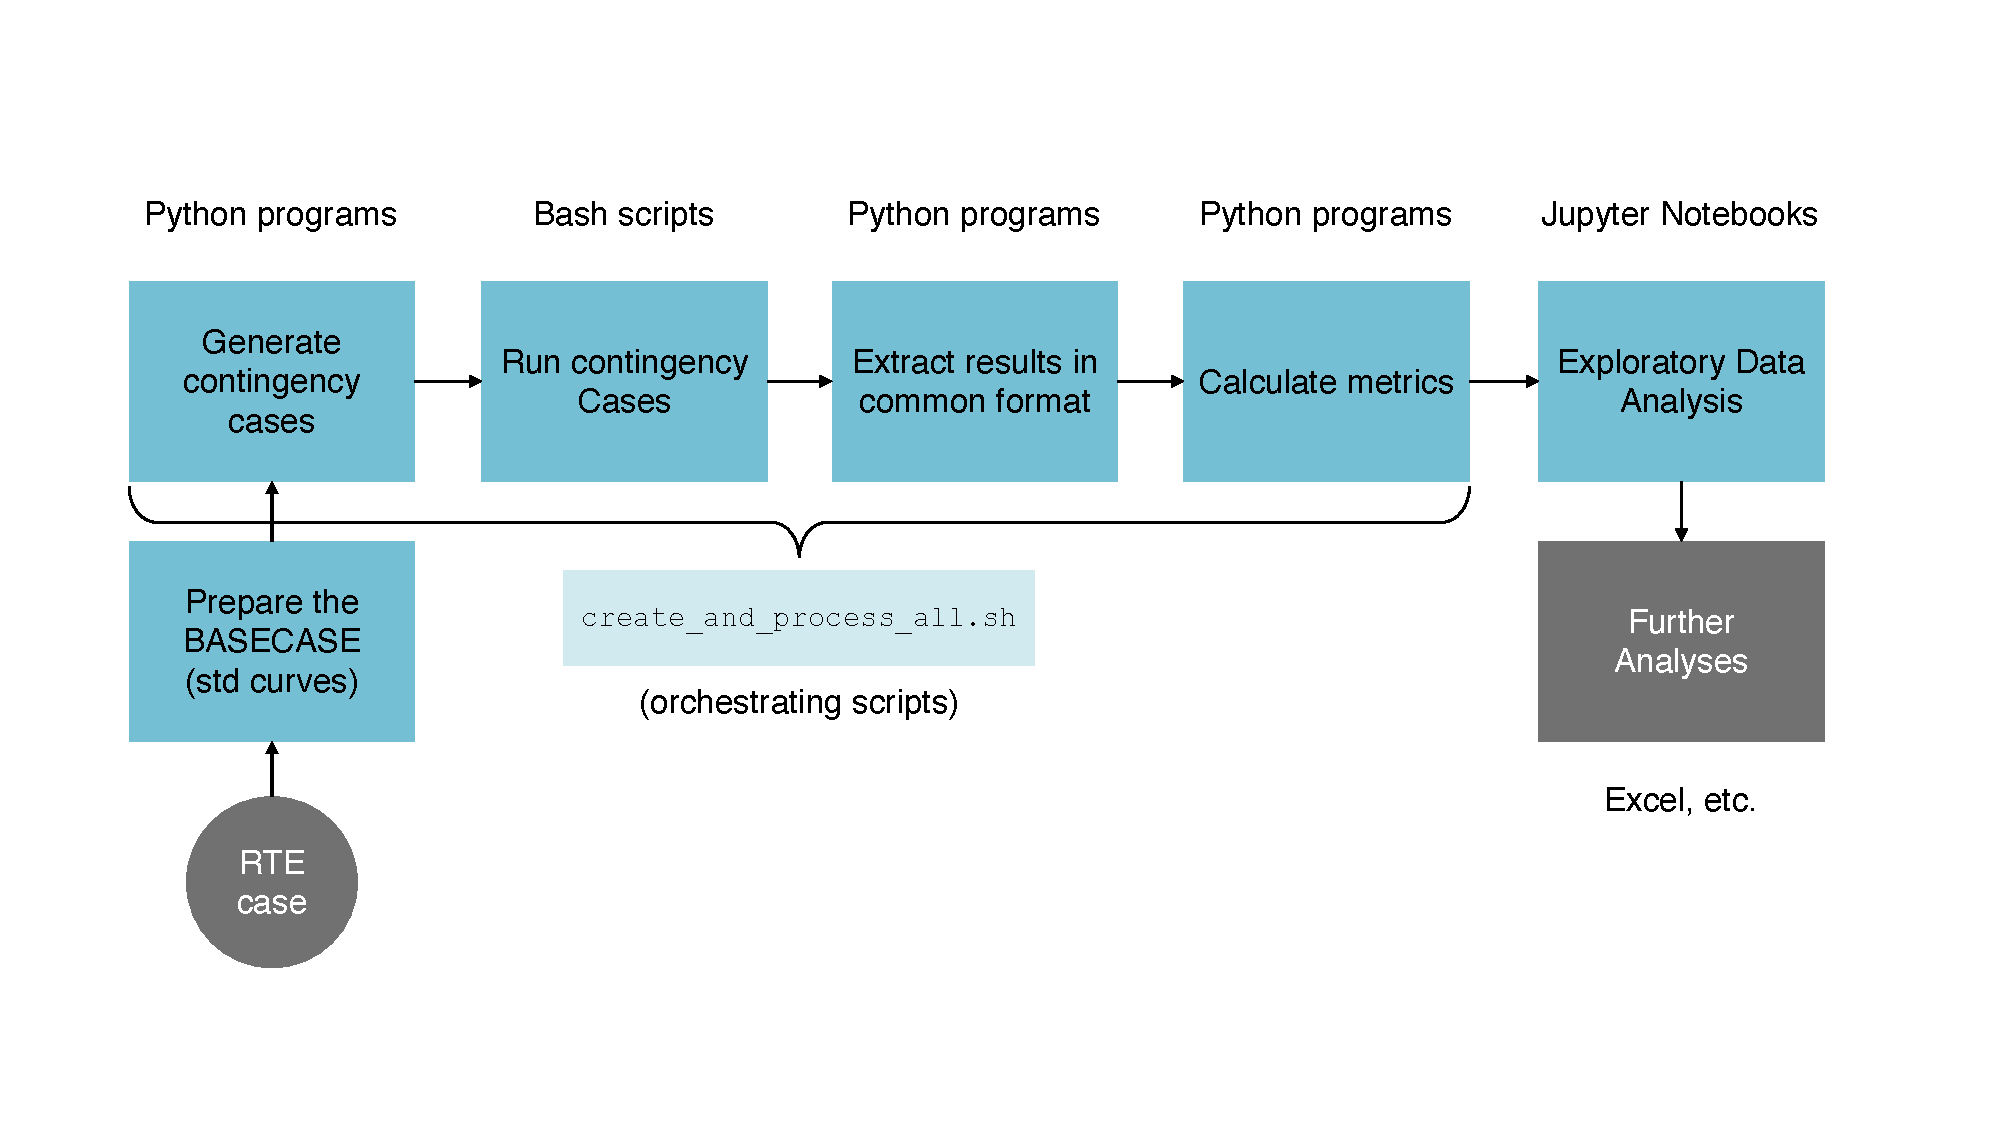
\includegraphics[width=0.48\textwidth]{figs/pipeline1}
  \caption{The processing pipeline for validating DynaWaltz/DynaFlow against
    Astre/Hades 2, based on contingency cases.}
  \label{fig:pipeline1}
\end{figure}

In terms of input, the system requires a valid case, in which the Astre/Hades 2 and
DynaWaltz/DynaFlow should obviously correspond to the same grid model and steady state.
They should be arranged with the following directory structure and file names:
\begin{console}
  <INPUTCASE_DIRNAME>
  |-- Astre
  |   `-- donneesModelesEntree.xml
  |-- fic_JOB.xml
  |-- t0
  |   |-- fic_CRV.xml
  |   |-- fic_DYD.xml
  |   |-- fic_IIDM.xml
  |   `-- fic_PAR.xml
  `-- tFin
  |-- fic_CRV.xml
  |-- fic_DYD.xml
  |-- fic_IIDM.xml
  `-- fic_PAR.xml
\end{console}

The directory file names should be exactly these, otherwise there will be
several parts of the pipeline that will fail. The parent directory name is free
(it's usually the date-time of the case).

Additionally, the system expects the input case (both in Astre/Hades 2 and DynaWaltz/DynaFlow) to
contain at least one disconnection event, since this is used as the reference to
obtain the time of the event. In other words, the scripts read
\code{"event\_tEvent"} and \code{"instant"} from the files, instead of
hard-coding the typical value (which is t=300 s). This time is read from the
first event, and then all events are discarded and replaced with the new
contingency event.






\subsection{Details for DynaFlow}
\begin{center}
  \itshape
  Outline:
  \begin{itemize}
    \item Preparing the base case: points to note. A/B case preparation.
    \item Running the cases: points to note
    \item Directory structure of the results
    \item Notebook: where they are created.
  \end{itemize}
\end{center}


\subsection{Details for DynaWaltz}
\begin{center}
  \itshape
  Outline:
  \begin{itemize}
    \item Preparation of the basecase, points to note:
          \begin{itemize}
            \item xml\_format
            \item preparation of curves, etc.
            \item t0, tFin stages (and the finalState dump, common to all runs)
          \end{itemize}
    \item Directory structure of the results
    \item Notebook: where they are created
    \item Discuss briefly the difficulties involved in making sure we're
          configuring the same event in Astre vs DynaWaltz.
    \item Discuss briefly some of the difficulties encountered, as in the
          case of NODE\_BREAKER vs BUS\_BREAKER w.r.t. bus contingencies.
  \end{itemize}
\end{center}



%%%%%%%%%%%%%%%%%%%%%%%%%%%%%%%%%%%%%%%%%%%%%%%%%%%%%%%%%%%%%%%%%%%%%%%%%%%%%%%%
\section{Metrics}
\begin{center}
  \itshape
  Outline:
  \begin{itemize}
    \item DynaFlow: design decisions for the metrics selected.
    \item DynaWaltz: design decisions for the metrics selected. Details of
          the key magnitudes extracted from curve signals (peak-to-peak
          amplitude, transient length, etc.)
    \item \textbf{Fig} of the metrics designed for comparing curves in the
          DynaWaltz tool.
  \end{itemize}
\end{center}




%%%%%%%%%%%%%%%%%%%%%%%%%%%%%%%%%%%%%%%%%%%%%%%%%%%%%%%%%%%%%%%%%%%%%%%%%%%%%%%%
\section{Use cases}

\begin{center}
  \itshape  Outline:
  \begin{itemize}
    \item \TODO: select interesting cases
    \item DynaWaltz: cases where DynaWaltz and Astre differed in the
          reactive/active injection of some generators?
    \item DynaFlow: mention the problem of ensuring that the steady-state
          is really attained? (i.e. flagging instability), mentioning cascaded disconnections, modelling of SVarC that are different (U+Lambda*Q in DynaFlow, not in Hades), modelling of loads that can explain some differences (restorative loads with voltage limitations), special protection schemes in DynaFlow and not in Hades 2 (SMACC, ACMC, ADA, etc.)
    \item \textbf{Fig} of some graph from the Notebooks
  \end{itemize}
\end{center}


%%%%%%%%%%%%%%%%%%%%%%%%%%%%%%%%%%%%%%%%%%%%%%%%%%%%%%%%%%%%%%%%%%%%%%%%%%%%%%%%
\section{Installation and usage}
\begin{center}
  \itshape Outline:
  \begin{itemize}
    \item Just a short description. See the Github repo for all the gory
          details.
    \item Facilitated installation via standard Python packaging
          infrastructure: pip, PyPI.
    \item We did not use an application installer because these tools are
          closer to a library than to a stand-alone monolithic application; We
          want to promote further development and easy customization.
    \item On top of a standard bare-bones Python 3 environment, the
          required third-party packages will add up to around 450 MB
          (it will be considerably less if you already have some of the
          largest packages, such as Pandas or Plotly.)
  \end{itemize}
\end{center}



%%%%%%%%%%%%%%%%%%%%%%%%%%%%%%%%%%%%%%%%%%%%%%%%%%%%%%%%%%%%%%%%%%%%%%%%%%%%%%%%
\section{Conclusion}

\begin{center}
  \itshape Outline:
  \begin{itemize}
    \item validation of dyn simulators is hard; you need large-network
          functional testing (i.e. not only individual element models in isolation)
    \item but also need a means to explore the effects of different model
          choices, model parameters, solver parameters, etc. on the behavior
          of the whole network.
    \item also for testing new versions of the software (i.e. as a
          complement to Unit Testing)
    \item This enables establishing an ongoing testing procedure to keep
          evolving the software, the models, and their parameterization.
    \item these tools presented here leverage modern rapid development
          tools from the Python ecosystem (Pandas, Jupyter Notebooks) to
          accomplish this. Can automatically configure extensive sets of test
          case and manage large amounts of output
    \item to be released as Open Source under the Dyna$\omega$o project
          repo. Easily customizable and extensible.
  \end{itemize}
\end{center}




%%%%%%%%%%%%%%%%%%%%%%%%%%%%%%%%%%%%%%%%%%%%%%%%%%%%%%%%%%%%%%%%%%%%%%%%%%%%%%%%
\section*{Acknowledgment}

\TODO We thank...  (RTE, Linux Foundation Energy?)

Lorem ipsum~\cite{Fabozzi09} dolor sit amet~\cite{Fabozzi11}, consectetur
adipiscing elit. Pellentesque neque arcu, pellentesque vel metus sed, semper
efficitur diam. Nulla tortor tortor, efficitur non accumsan vel, dignissim vitae
risus. Fusce sit amet nibh eget ante consequat pretium. Donec vel nulla vitae
sapien aliquet semper eget ut enim. In ultrices blandit metus, vel ultrices
sapien pretium id. Maecenas tincidunt egestas nibh, at sodales metus blandit
a. Integer auctor consequat mauris, non luctus erat tincidunt vitae. Integer
accumsan dapibus metus, ut posuere felis cursus vitae. Quisque vulputate dui
quis turpis auctor, at rutrum nibh fermentum. Quisque eu elit eu mi molestie
pulvinar id vitae sapien.




%%%%%%%%%%%%%%%%%%%%%%%%%%%%%%%%%%%%%%%%%%%%%%%%%%%%%%%%%%%%%%%%%%%%%%%%%%%%%%%%
\bibliographystyle{IEEEtran}
\bibliography{IEEEabrv,dynawo_validation}




\end{document}




%% Place figures and tables at the top and bottom of columns. Avoid placing them in
%% the middle of columns. Large figures and tables may span across both
%% columns. Figure captions should be below the figures; table heads should appear
%% above the tables. Insert figures and tables after they are cited in the
%% text. Use the abbreviation ``Fig.~\ref{fig}'', even at the beginning of a
%% sentence.
%%
%% \begin{table}[htbp]
%%   \caption{Table Type Styles}
%%   \begin{center}
%%     \begin{tabular}{|c|c|c|c|}
%%       \hline
%%       \textbf{Table}&\multicolumn{3}{|c|}{\textbf{Table Column Head}} \\
%%       \cline{2-4} 
%%       \textbf{Head} & \textbf{\textit{Table column subhead}}&
%%       \textbf{\textit{Subhead}}& \textbf{\textit{Subhead}} \\
%%       \hline
%%       copy& More table copy$^{\mathrm{a}}$& &  \\
%%       \hline
%%       \multicolumn{4}{l}{$^{\mathrm{a}}$Sample of a Table footnote.}
%%     \end{tabular}
%%     \label{tab1}
%%   \end{center}
%% \end{table}

%% \begin{figure}[htbp]
%%   \centerline{\includegraphics{fig1.png}}
%%   \caption{Example of a figure caption.}
%%   \label{fig}
%% \end{figure}

